\chapter{Recurrencias y los métodos para resolverlas}

Una \textbf{recurrencia} es una función expresada en términos de sí misma, pero con una entrada más pequeña. 
Las recurrencias se presentan comúnmente durante el análisis de la eficiencia de un algoritmo. 
La \textbf{forma cerrada} de una recurrencia es una función equivalente, pero expresada sin recursividad. 
Para resolver una recurrencia, se debe encontrar su forma cerrada.

\marginnote[1\baselineskip]{%
  Cabe mencionar que el tamaño de los subproblemas no necesariamente es siempre una fracción del problema original; una recurrencia puede reducir el tamaño de la entrada de diferentes formas.
}

En el contexto de los algoritmos \emph{divide y vencerás}, las recurrencias tienen la sig. forma general: 
\[
  T(n)=\begin{cases}
    \sum_{i=1}^pT(n_i)+f(n)+g(n) & \text{si }n>b\\
    h(n) & \text{si } n=b
  \end{cases}
\]
donde

\begin{itemize}
  \item \(b\in\mathbb{N}\) es la \textbf{condición de paro}; esto es, el valor que debe tener \(n\) para entrar al \textbf{caso base} de la recurrencia.
  \item \(p\in\mathbb{N}\) es la cantidad de subproblemas en que se divide la entrada en cada llamada recursiva.
  \item \(n_i\in\mathbb{N}\), tal que \(n_i<n\), es el tamaño de la entrada
  para el subproblema \(i\).
  \item \(f:\mathbb{N}\to\mathbb{N}\) es el tiempo de ejecución requerido para dividir la entrada en \(p\) subproblemas.
  \item \(g:\mathbb{N}\to\mathbb{N}\) es el tiempo de ejecución requerido para combinar las soluciones de los \(p\) subproblemas.
  \item \(h:\mathbb{N}\to\mathbb{N}\) es el tiempo de ejecución requerido para resolver el caso base de la recurrencia; esto es, cuando la entrada es lo suficientemente pequeña para resolver el problema sin necesidad de dividirlo en subproblemas. 
\end{itemize}

Sin embargo, en la práctica, las recurrencias se escriben de una forma más simple.
Primero, el caso base de un algoritmo por lo general se alcanza cuando \(n\) es de un tamaño pequeño determinado que puede procesarse en tiempo constante; es decir, lo más común es que \(h(n)=\Theta(1)\).
Debido a esto, \(h(n)\) suele omitirse.
Segundo, lo más común es que un algoritmo requiera tiempo constante únicamente para dividir el problema o para combinar las soluciones parciales; es decir, ya sea \(f(n)=\Theta(1)\) o \(g(n)=\Theta(1)\), pero no ambos al mismo tiempo.
Además, rara vez ocurre que ambas acciones requieren cada una un tiempo mayor a \(\Theta(1)\).
Debido a esto, suele escribirse solo una función, \(f(n)\), en lugar de dos.
Así, las recurrencias comúnmente se escriben simplemente como
\[
  T(n)=\sum_{i=1}^pT(n_i)+f(n).
\]

Finalmente, los pisos y los techos también suelen omitirse en las recurrencias y, en cambio, suele suponerse que \(n\) siempre es lo suficientemente grande para dividirlo en partes enteras.
Así, en lugar de escribir \(T(\lceil n/2 \rceil)+T(\lfloor n/2 \rfloor)\), simplemente se escribe \(2T(n/2)\).
A pesar de que hacer esto puede cambiar la solución exacta de la recurrencia, generalmente solo lo hace en un factor constante y el comportamiento asintótico de la recurrencia no cambia.

\section{El método del árbol recursivo}

El método del árbol recursivo es un método gráfico e informal para resolver recurrencias y consiste en dibujar un árbol donde cada nodo representa el tiempo requerido para resolver un subproblema.
Al sumar el valor de todos los nodos del árbol, se puede obtener la forma cerrada de la recurrencia. 
Antes de estudiar el método en sí, es importante recordar algunos conceptos sobre árboles.

Sea \(k\in\mathbb{N}\), un \textbf{árbol} \(\boldsymbol{k}\)\textbf{-ario} es un árbol enraizado donde cada nodo tiene a lo más \(k\) hijos. 
Un árbol \(k\)-ario \textbf{lleno} es aquél donde cada nodo es una hoja o tiene exactamente \(k\) hijos. 
La \textbf{profundidad} de un nodo es la distancia más corta entre dicho nodo 
y la raíz. 
Por definición, la raíz tiene una profundidad de 0.
Un árbol \(k\)-ario \textbf{completo} es un árbol lleno donde todas las hojas tienen la misma profundidad.
En un árbol \(k\)-ario completo, el número de nodos a profundidad \(d\) está dado por \(k^d\).
La \textbf{altura} de un árbol es la profundidad más grande de todos los nodos.
Así, la altura de un árbol \(k\)-ario completo con \(n\) hojas está dado por \(\log_k{n}\).
Finalmente, el número de nodos internos en un árbol \(k\)-ario completo de altura \(h\) está dado por
\[
  1+k+k^2+\dots+k^{h-1} = 
  \sum_{d=0}^{h-1}k^d =
  \sum_{d=1}^{h}k^d =
  \dfrac{k^h-1}{k-1}.
\]

El método del árbol recursivo consta de los sig. pasos:

% \marginnote[1.5\baselineskip]{%
%   Las expresiones obtenidas en los pasos 2, 3 y 4 se definen en función de \(n\) y la expresión obtenida en el paso 5 normalmente consta de una sumatoria que debe resolverse para obtener la forma cerrada.
% }

\begin{enumerate}
  \item Se dibuja el árbol recursivo de la recurrencia cumpliendo con las sig. características:
  \begin{itemize}
    \item La raíz contiene la expresión \(f(n)\).
    \item Cada nodo interno contiene la expresión \(f(n_i)\).
    \item Cada hoja contiene la expresión \(h(n)\), q. casi siempre es \(\Theta(1)\).
    \item Cada nodo interno tiene \(p\) hijos.
  \end{itemize}
  \item Se calcula la altura del árbol; esto es, la ruta más larga que sigue el algoritmo en el árbol para llegar al caso base.
  \item Se calcula la cantidad de hojas; esto es, el número de nodos en el nivel más profundo.
  \item Se suman los valores de todos los nodos por cada nivel.
  \item Se suman los resultados de todos los niveles, obtenidos en el paso anterior.
  \item Se resuelve la expresión resultante para obtener la forma cerrada.
\end{enumerate}

\begin{figure*}[t]
  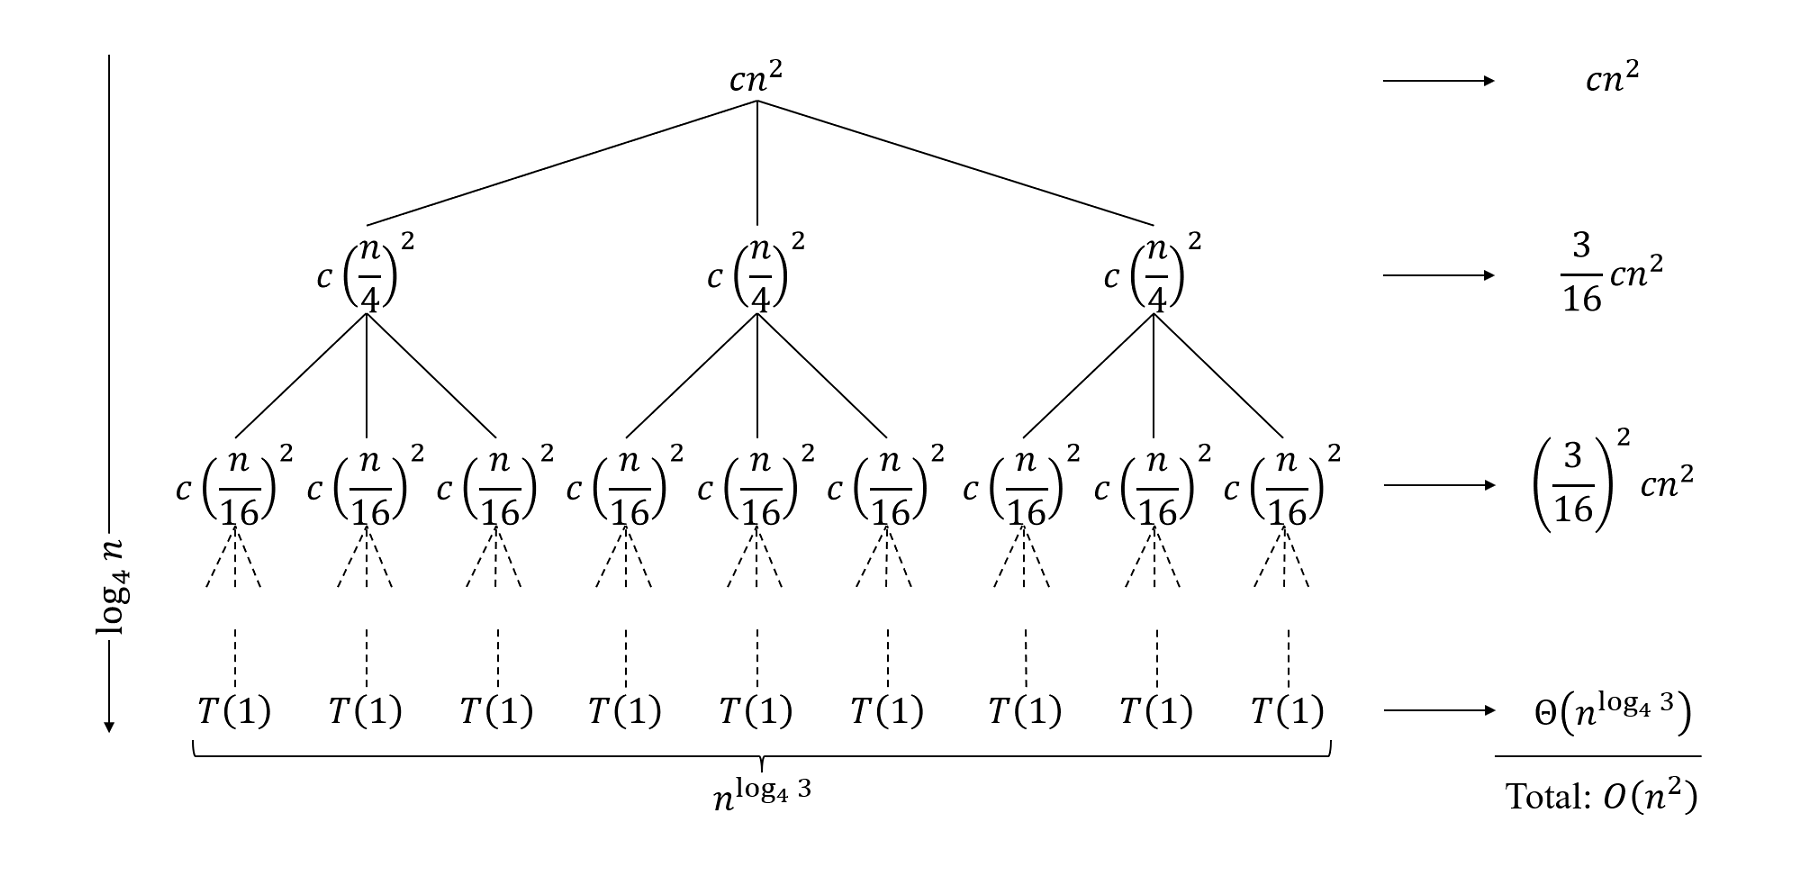
\includegraphics[width=1\textwidth]{figuras/recursion-tree.png}
  \caption{Usando el método del árbol recursivo para resolver la recurrencia \(T(n)=3T(n/4)+cn^{2}\).}
  \label{fig:recursion_tree}
\end{figure*}

\begin{expl}
  Considérese la recurrencia \(T(n)=3T(n/4)+\Theta(n^2)\). 
  Antes de comenzar, se debe sustituir \(\Theta(n^2)\) por \(cn^2\), donde \(c\in\mathbb{R}^+\) es una constante. 
  Así, se simplifica la recurrencia como \(T(n)=3T(n/4)+cn^2\). 
  El sig. paso es dibujar el árbol recursivo, el cual se muestra en la Figura \ref{fig:recursion_tree}.
  
  Después, se debe calcular la altura del árbol. 
  Dado que el valor de \(n\) se reduce en un factor de \(1/4\) en cada nivel, la altura es el número de niveles que deben de recorrerse hasta llegar a 1. Así, la altura \(h\) puede calcularse como
  \[
    \begin{aligned}
      \left(\dfrac{1}{4}\right)^h\cdot n &= 1 \\
      \dfrac{1}{4^h}\cdot n &= 1 \\
      n &= 4^h \\
      \log_4{n} &= h.
    \end{aligned}
  \]
  
  Luego, se debe calcular el número de hojas; esto es, el número de nodos en el nivel más profundo.
  Dado que cada nodo tiene exactamente 3 hijos Esto está dado por
  \[
    3^h = 3^{\log_4{n}} = n^{\log_4{3}}.
  \]
  
  El siguiente paso es calcular el tiempo total de cada nivel.
  En la Figura \ref{fig:recursion_tree}, se observa que de dicha suma surge un patrón que se repite en función de \(cn^2\).
  En cuanto a la suma del último nivel, dado que el tiempo requerido por el caso base está dado por \(T(1)=\Theta(1)\), dicha suma es igual al número de hojas, que ya se calculó.
  
  Por último, se suman los tiempos de todos los niveles, lo que resulta en la sig. expresión:
  
  \begin{align*}
    T(n)&=\sum_{i=0}^{\log_{4}n-1}\left(\dfrac{3}{16}\right)^{i}\cdot cn^{2}+\Theta(n^{\log_{4}3}) \\
    &<\sum_{i=0}^{\infty}\left(\dfrac{3}{16}\right)^{i}\cdot cn^{2}+\Theta(n^{\log_{4}3}) \\
    &=\dfrac{1}{1-3/16}\cdot cn^{2}+\Theta(n^{\log_{4}3}) \\
    &=\dfrac{16}{13}\cdot cn^{2}+\Theta(n^{\log_{4}3}) \\
    &=O(n^{2})+O(n^{\log_{4}3}) \\
    &=O(n^{2}).
  \end{align*}
	\exend
\end{expl}

\section{El método de sustitución}

El método de sustitución es un método formal que consiste en resolver una recurrencia utilizando inducción matemática. 
Específicamente, este método consta de los sig. pasos:
\begin{enumerate}
  \item Se propone una cota asintótica como la solución tentativa de la recurrencia.
  \item Se utiliza inducción para demostrar que la recurrencia sí cumple con la cota propuesta y para encontrar las constantes de dicha cota.
\end{enumerate}
Este método se puede utilizar para calcular tanto una cota superior como una inferior.

\paragraph{Para proponer una buena solución tentativa.}{%
  Se puede utilizar el método del árbol recursivo para obtener una solución tentativa.
  Después, se puede usar el método de sustitución para demostrar que dicha solución es correcta o para ajustar la cota en caso de que no lo sea.
  Otra alternativa es que, si la recurrencia tiene una forma similar a alguna otra cuya solución ya se conoce, se puede proponer esa solución como la solución tentativa.
  Como último recurso, se pueden proponer dos cotas holgadas, una inferior y  una superior, y ajustarlas gradualmente hasta que converjan en la solución correcta. 
}
\paragraph{Diferencias con la inducción matemática.}{%
  El caso base se demuestra hasta el final y no al principio de la demostración.
  La hipótesis inductiva consiste en suponer que la cota se cumple para cualquier subproblema, \(T(n_i)\), donde \(n_i<n\). 
  El paso inductivo consiste en sustituir \(T(n_i)\) (en la recurrencia original) por la forma exacta de la cota propuesta en la hipótesis inductiva. 
  Este paso da origen al nombre del método.
}
\paragraph{Cuidado con la notación asintótica.} {%
  El objetivo del método de sustitución es demostrar algebraicamente que 
  la cota propuesta se cumple de \emph{forma exacta}.
  Es incorrecto aplicar la notación asintótica en el paso inductivo para deshacerse de constantes o términos problemáticos.
}
\paragraph{Cuando la cota propuesta es correcta pero la inducción no converge a ella.}
{%
  En lugar de proponer una cota más holgada, se puede proponer una nueva hipótesis inductiva, cuya única diferencia con la hipótesis original es que se resta un término de grado menor a la cota propuesta.
}

\begin{expl}
  \label{ex:recurrence_substitution}
  Considérese la recurrencia \(T(n)=2T(\lfloor n/2 \rfloor)+n\) y supóngase que se propone \(O(n\lg{n})\) como la solución tentativa. 
  Entonces, se busca demostrar que \(T(n)\leq cn\lg{n}\) para alguna constante \(c>0\).
  \begin{description}
    \item[Hipótesis inductiva] Supóngase que \(T(\lfloor n/2\rfloor)\leq c\lfloor n/2\rfloor\lg\lfloor n/2\rfloor\).
    \item[Paso inductivo] Sustituyendo la hipótesis inductiva en la recurrencia original, se tiene:
    \begin{align*}
      T(n) &\leq2c\lfloor n/2\rfloor\lg\lfloor n/2\rfloor+n \\
      &\leq cn\lg(n/2)+n \\
      &=cn\lg n-cn\lg2+n \\
      &=cn\lg{n}-cn+n \\
      &\leq cn\lg n.
    \end{align*}
    Aparentemente, la solución propuesta es la correcta (para toda \(c\geq 1\)). 
    Sin embargo, hace falta demostrar que esta solución también se cumple para la condición de paro de la recurrencia. 
    Esto debe demuestrarse por construcción; esto es, se debe encontrar un valor para \(c\) que satisfaga la cota en la condición de paro. 
    A continuación, se muestra cómo esto puede llevar a ciertos problemas. 
    \item[Caso base] Supóngase que \(T(1)=1\). 
    Aplicando la cota propuesta a la condición de paro, se tiene que \(T(1)\leq cn\lg n=c\lg{1}=0\), lo que contradice que \(T(1)=1\). 
    Por lo tanto, la solución propuesta falla en el caso base. 
    Sin embargo, hay que recordar que la definición de la notación asintótica requiere que la cota se cumpla únicamente para un valor de \(n\) mayor que algún umbral \(n_{0}\) que \emph{uno es libre de elegir a voluntad}. 
    Esto quiere decir que no es obligatorio utilizar la condición de paro de la recurrencia como el caso base de la inducción. 
    Para este ejemplo, obsérvese que \(T(\lfloor2/2\rfloor)=T(\lfloor3/2\rfloor)=T(1)\), por lo que se puede utilizar \(T(2)\) y \(T(3)\) como el caso base. 
    Esto es equivalente a elegir \(n_0=2\).
    Aplicando la hipótesis inductiva al nuevo caso base, se tiene:
    \begin{align*}
      T(2) & \leq 2c\lg2 & T(3) & \leq 3c\lg3 \\
      2T(\lfloor 2/2 \rfloor) + 2 & \leq 2c & 2T(\lfloor 3/2 \rfloor) + 3 & \leq 3c(1.585) \\
      2T(1) + 2 & \leq2c & 2T(1) + 3 & \leq 3c(1.585) \\
      4 & \leq 2c & 5 & \leq 3c(1.585) \\
      2 & \leq c, & \dfrac{5}{4.755} & \leq c.
    \end{align*}
    Por lo tanto, queda demostrado que \(T(n)\leq cn\lg{n}\) para toda \(c\geq 2\). \exend
  \end{description}
\end{expl}

\begin{expl}
    Considérese ahora la recurrencia \(T(n)=T(\lfloor n/2\rfloor)+T(\lceil n/2\rceil)+1\) y supóngase que se propone \(O(n)\) como la solución tentativa. 
    Se busca demostrar que \(T(n)\leq cn\) para alguna \(c>0\).
    \begin{description}
      \item[Hipótesis inductiva] Supóngase que \(T(\lfloor n/2\rfloor)\leq c\lfloor n/2\rfloor\) y que \(T(\lceil n/2\rceil)\leq c\lceil n/2\rceil\).
      \item[Paso inductivo] Sustituyendo la hipótesis inductiva en la recurrencia original, se tiene: \(T(n) \leq c\lfloor n/2 \rfloor + 1 = cn + 1\).
      Esto sugiere que la solución propuesta no es correcta.
      En este ejemplo, se ve que el término \(+1\) impide que la igualdad se cumpla de forma exacta.
      En lugar de proponer una cota más holgada, se propone une nueva hipótesis inductiva.
      \item[Nueva H.I.] Supóngase que \(T(\lfloor n/2\rfloor)\leq c\lfloor n/2\rfloor-d\) y que \(T(\lceil n/2\rceil)\leq c\lceil n/2\rceil-d\), donde \(d\in\mathbb{R}^+\).
      \item[Paso inductivo] Sustituyendo la hipótesis inductiva en la recurrencia original, se tiene lo sig.:
      \begin{align*}
        T(n) &\leq c\lfloor n/2\rfloor-d+c\lceil n/2\rceil-d+1\\
        &=cn-2d+1\\
        &\leq cn-d.
      \end{align*}
      Esto se cumple para toda \(d\geq 1\). 
      Ahora solo queda demostrar que la cota se cumple para la condición de paro.
      \item[Caso base] Obsérvese que \(n=2\) es el valor más pequeño que resulta en \(T(1)\), tanto para \(T(\lfloor n/2 \rfloor)\) como para \(T(\lceil n/2 \rceil)\). 
      Aplicando la hipótesis inductiva a estos términos, se tiene que:
      \begin{align*}
        T(2) &\leq 2c-d\\
        T(\lfloor 2/2 \rfloor) + T(\lceil 2/2 \rceil) + 1 &\leq 2c-d \\
        2T(1) + 1 &\leq 2c - d \\
        \dfrac{2T(1)+1+d}{2} &\leq c \\
        T(1) + \dfrac{1+d}{2} &\leq c.
      \end{align*}
      \exend
    \end{description}
\end{expl}

\section{El Teorema Maestro}

Un método para resolver recurrencias consiste simplemente en aplicar el sig. teorema.

\begin{thm}[\textbf{Teorema Maestro}]
  Sean \(a,b,n\in\mathbb{N}\), donde \(a\) y \(b\) son constantes y \(b>1\), sea \(f:\mathbb{N}\to\mathbb{N}\) una función asintóticamente positiva y sea \(c=\log_{b}a\). 
  La recurrencia \(T(n)=aT(n/b)+f(n)\) puede resolverse aplicando uno de los sig. casos:
  \begin{enumerate}
    \item Si \(f(n)=O(n^{c-\varepsilon})\) para alguna constante real $\varepsilon>0$, entonces \(T(n)=\Theta(n^{c})\).
    \item Si \(f(n)=\Theta(n^c)\), entonces \(T(n)=\Theta(n^{c}\log{n})\).
    \item Si \(f(n)=\Omega(n^{c+\varepsilon})\) y si, además, \(af(n/b)\leq kf(n)\) para alguna constante real \(k<1\) y para todo valor de \(n\) mayor que algún umbral, entonces \(T(n)=\Theta(f(n))\).
  \end{enumerate}
\end{thm}

\begin{rem}
  En el Teorema Maestro, el término \(n/b\) de la recurrencia \(T(n)\) también puede interpretarse como \(\lceil n/b\rceil\) o \(\lfloor n/b\rfloor\).
\end{rem}

Intuitivamente, la recurrencia \(T(n)\) sobre la que puede aplicarse el Teorema Maestro describe un algoritmo que divide el problema en \(a\) subproblemas \emph{del mismo tamaño}, donde, en cada subproblema, el tamaño de la entrada se reduce en un factor de \(1/b\), y donde se requiere \(f(n)\) tiempo de ejecución para dividir el problema y/o combinar las soluciones parciales.
Así, la función \(n^c\), descrita en el Teorema Maestro, representa el número de hojas en el árbol recursivo que representa a esta recurrencia.

El Teorema Maestro indica que, comparando \(n^c\) con \(f(n)\), la función que crece más rápido acota el tiempo de ejecución del algoritmo en cuestión.
En el caso 1, se tiene que \(n^c\) crece más rápido; esto es, el tiempo requerido para resolver cada subproblema eventualmente supera el tiempo requerido por la división y/o combinación.
Por ende, en este caso \(n^c\) acota la solución de la recurrencia.
En el caso 3, se tiene lo opuesto; \(f(n)\) crece más rápido que \(n^c\).
Para aplicar este caso, \(f(n)\) debe además satisfacer lo que se conoce como
la \textbf{condición de regularidad}.
Por último, en el caso 2, se tiene que ambas funciones, \(f(n)\) y \(n^c\), tienen el mismo orden de crecimiento y, por ende, la solución es dicho orden multiplicado por un factor logarítmico que representa la altura del árbol recursivo.

\begin{expl}
  Sea $T(n)=9T(n/3)+n$. Aplicando el Teorema Maestro, se tiene que \(a=9\), 
  \(b=3\) y \(f(n)=n\). 
  Así, se obtiene \(n^c=n^{\log_{3}{9}}=n^2\). 
  Dado que \(f(n)=O(n^{2-\varepsilon})\), donde \(\varepsilon=1\), se puede aplicar el caso 1, lo que resulta en que \(T(n)=\Theta(n^2)\). \exend
\end{expl}

\begin{expl}
  Sea \(T(n)=T(2n/3)+1\). 
  Aplicando el Teorema Maestro, se tiene que \(a=1\), \(b=3/2\) y \(f(n)=1\). 
  Así, se obtiene \(n^c=n^{\log_{3/2}{1}}=n^0=1\).
  Dado que \(f(n)=n^c=1\), se puede aplicar el caso 2, lo que resulta en \(T(n)=\Theta(\log{n})\). \exend
\end{expl}

\begin{expl}
  Sea \(T(n)=3T(n/4)+n\lg{n}\). 
  Aplicando el Teorema Maestro, se tiene que \(a=3\), \(b=4\) y \(f(n)=n\lg{n}\). 
  Así, se obtiene \(n^c=n^{\log_{4}{3}}=O(n^{0.793})\). 
  Dado que \(f(n)=\Omega(n^{\log_{4}{3}+\varepsilon})\), donde \(\varepsilon\approx 0.2\), se puede aplicar el caso 3 si se demuestra 
  que \(af(n/b)\leq kf(n)\), donde \(k<1\). 
  Para ello, se tiene que \(3(n/4)\lg(n/4)\leq (3/4)n\lg{n}\) para valores suficientemente grandes de \(n\). 
  Como consecuencia, se puede aplicar el caso 3, lo que resulta en \(T(n)=\Theta(n\log n)\). \exend
\end{expl}

\begin{expl}
  Sea \(T(n)=2T(n/2)+n\lg{n}\). 
  El Teorema Maestro no se puede aplicar a esta recurrencia a pesar de tener la forma apropiada. 
  Si se maneja que \(a=2\), \(b=2\) y \(f(n)=n\lg{n}\), se obtendría \(n^c=n^{\log_{2}{2}}=n\).
  Dado que \(f(n)\) es asintóticamente más grande que \(n^c\), se podría pensar que se puede aplicar el caso 3, pero no es así debido a que \(f(n)\) no es
  mayor que \(n^c\) en un factor polinomial. \exend
\end{expl}

\section{Cambio de variable}

En ocasiones, se puede aplicar álgebra para transformar una recurrencia en alguna otra cuya solución ya se conoce, eliminando la necesidad de recurrir a cualquiera de los métodos anteriores.

\begin{expl}
  Sea \(T(n)=2T(\lfloor \sqrt{n} \rfloor)+\lg{n}\). Esta recurrencia se 
  puede simplificar con un cambio de variable. 
  Proponiendo que \(m=\lg{n}\), se tiene que \(T(2^m)=2T(2^{m/2})+m\). 
  Si además se propone una función \(S(m)=T(2^m)\), se obtiene la recurrencia \(S(m)=2S(m/2)+m\), que es idéntica a la recurrencia resuelta en el ejemplo \ref{ex:recurrence_substitution}, por lo que la solución es la misma para ambas. 
  Entonces, \(S(m)=O(m\lg m)\). 
  Cambiando de regreso \(S(m)\) por \(T(n)\), se obtiene \(T(n)=O(\lg{n}\cdot\lg\lg{n})\). \exend
\end{expl}

\section{Notas bibliográficas}

En el libro de \textcite{cormen_2009}, págs. 97-106, se proporciona la demostración del Teorema Maestro.
Además, en las págs. 112-113, se describe el \textbf{método de Akra-Bazzi} \citep{akra_1998,leighton_1996}, que se utiliza para resolver recurrencias donde el problema se divide en subproblemas que difieren mucho de tamaño.
Este método trabaja con variables contínuas.
Por otro lado, \textcite{drmota_2013} presentan una especialización del método de Akra-Bazzi que trabaja con variables discretas. 

\marginnote[-1\baselineskip]{%
  \textbf{Literatura consultada}: \textcite{cormen_2009} pp. 65-67, 83-97.
}
